\chapter{Hartree--Fock: ý tưởng trường trung bình}
\label{ch:hf}

\section{Ý tưởng: thay ``đám đông thật'' bằng ``đám đông trung bình''}

\begin{eli5}[sàn nhảy đông người]
Bạn nhảy trên một sàn nhảy đông người. Liên tục né từng người cụ thể thì quá phức tạp, nên bạn chỉ cảm nhận ``mật độ đám đông trung bình'': chỗ nào thường đông thì tránh, chỗ nào thưa thì tới. Mọi người khác cũng làm y như vậy. Nhưng ``đám đông trung bình'' lại do chính mọi người tạo ra, nên cả nhóm phải điều chỉnh qua lại cho tới khi bức tranh ổn định: không ai muốn đổi chỗ nữa. Đó là ý tưởng \textbf{trường trung bình} \en{mean field} và \textbf{trường tự hợp} \en{self-consistent field, SCF}.

\emph{Chỗ ví dụ ``gãy'':} người thật né nhau \emph{tức thời} (thấy người kia lao tới thì tránh). Mô hình trung bình bỏ mất điều đó, và phần bị bỏ mất chính là năng lượng tương quan.
\end{eli5}

Ý tưởng này biến bài toán $N$ electron dính chùm thành $N$ bài toán một electron, mỗi bài toán là một electron chuyển động trong ``trường'' của hạt nhân cộng với đám mây trung bình của các electron còn lại. Bài toán một electron thì ta giải được.

\subsection{Phương pháp Hartree (1928)}
Năm 1928, Douglas Hartree giả thiết hàm sóng là tích Hartree $\Psi=\phi_1(\vr_1)\phi_2(\vr_2)\phi_3(\vr_3)$, và mỗi orbital thỏa \cite{Hartree1928a}
\[
\Big[-\tfrac12\nabla^2-\frac{Z}{r}+\sum_{j\neq i}\int\frac{|\phi_j(\vr')|^2}{|\vr-\vr'|}\,d\vr'\Big]\phi_i(\vr)=\varepsilon_i\,\phi_i(\vr).
\]
Số hạng tích phân là thế tĩnh điện do ``đám mây điện tích'' $|\phi_j|^2$ của các electron \emph{khác} tạo ra. Vì thế này phụ thuộc vào chính các orbital cần tìm, ta phải lặp: đoán orbital, tính thế, giải phương trình được orbital mới, rồi lặp lại cho tới khi ``trường vào bằng trường ra''. Hartree gọi đó là \emph{self-consistent field}.

Thiếu sót của Hartree: tích Hartree không phản đối xứng (chương~\ref{ch:hatdongnhat}). Năm 1930, Fock và Slater độc lập sửa lỗi này bằng cách thay tích Hartree bằng định thức Slater \cite{Fock1930,Slater1930}. Kết quả là phương pháp \textbf{Hartree--Fock} (HF). Li là một trong những nguyên tử đầu tiên được tính bằng HF đầy đủ: Fock và Petrashen, năm 1935.

\section{Phương trình Hartree--Fock}

Phương pháp HF tìm \emph{định thức Slater tốt nhất}: chọn các orbital sao cho năng lượng $E=\langle\Psi_0|\Hhat|\Psi_0\rangle$ nhỏ nhất. Theo nguyên lý biến phân, $\EHF\ge E_{\text{chính xác}}$.

\begin{congthuc}[năng lượng HF của Li]
Với định thức $|1s\!\uparrow\,1s\!\downarrow\,2s\!\uparrow|$ (orbital 1s dùng chung cho hai spin, gọi là ROHF), áp dụng quy tắc Slater--Condon \cite{Szabo1996}:
\[
E_{\rm HF}(\text{Li})=2h_{1s}+h_{2s}+J_{1s1s}+2J_{1s2s}-K_{1s2s}.
\]
\begin{itemize}
\item $h_{a}=\int\phi_a^*(\vr)\big[-\tfrac12\nabla^2-\tfrac{Z}{r}\big]\phi_a(\vr)\,d\vr$: động năng cộng hút hạt nhân của một electron ở orbital $a$.
\item $J_{ab}=\iint\dfrac{|\phi_a(\vr_1)|^2\,|\phi_b(\vr_2)|^2}{r_{12}}\,d\vr_1d\vr_2$: \textbf{tích phân Coulomb}, lực đẩy tĩnh điện giữa hai đám mây điện tích $|\phi_a|^2$ và $|\phi_b|^2$. Có ý nghĩa cổ điển rõ ràng.
\item $K_{ab}=\iint\dfrac{\phi_a^*(\vr_1)\phi_b(\vr_1)\,\phi_b^*(\vr_2)\phi_a(\vr_2)}{r_{12}}\,d\vr_1d\vr_2$: \textbf{tích phân trao đổi}. Chỉ xuất hiện giữa hai electron \emph{cùng spin}. Không có tương tự cổ điển: nó là hệ quả của tính phản đối xứng.
\end{itemize}
Với Li: $J_{1s1s}$ là đẩy giữa hai electron 1s (khác spin, nên không có $K$); $2J_{1s2s}$ là electron 2s đẩy cả hai electron 1s; $-K_{1s2s}$ chỉ có một lần, cho cặp cùng spin 1s$\uparrow$--2s$\uparrow$.
\end{congthuc}

\begin{congthuc}[toán tử Fock]
Cực tiểu hóa năng lượng (với ràng buộc các orbital trực chuẩn) dẫn tới phương trình trị riêng cho từng spin-orbital:
\[
\hat f\,\chi_a=\varepsilon_a\,\chi_a,\qquad \hat f=\underbrace{-\tfrac12\nabla^2-\frac{Z}{r}}_{\hat h}+\sum_{b}\big[\hat J_b-\hat K_b\big].
\]
\begin{itemize}
\item $\hat J_b\chi_a(\vr_1)=\Big[\int\frac{|\chi_b(\vx_2)|^2}{r_{12}}d\vx_2\Big]\chi_a(\vr_1)$: nhân với thế tĩnh điện của electron $b$. Toán tử \emph{cục bộ}: giá trị tại $\vr_1$ chỉ cần biết $\chi_a$ tại $\vr_1$.
\item $\hat K_b\chi_a(\vr_1)=\Big[\int\frac{\chi_b^*(\vx_2)\chi_a(\vx_2)}{r_{12}}d\vx_2\Big]\chi_b(\vr_1)$: ``tráo'' nhãn $a\leftrightarrow b$. Toán tử \emph{phi cục bộ}: cần biết $\chi_a$ trên toàn không gian.
\item $\varepsilon_a$: \textbf{năng lượng orbital}.
\end{itemize}
Vì $\hat J_a\chi_a=\hat K_a\chi_a$, số hạng $b=a$ tự triệt tiêu: \textbf{electron không tự đẩy chính mình}. Đây là một ưu điểm của HF mà ta sẽ nhắc lại khi nói về lỗi ``tự tương tác'' của DFT (chương~\ref{ch:dft}).
\end{congthuc}

\begin{eli5}[trao đổi]
Hai electron cùng spin giống hai cầu thủ cùng áo bị luật chơi cấm đứng chung một chỗ. Không ai đẩy ai, nhưng quanh mỗi người vẫn có một ``vùng cấm'' với đồng đội (lỗ Fermi). Vì tự động đứng xa nhau hơn, lực đẩy trung bình giữa họ nhỏ đi, nên năng lượng giảm một lượng $K$. Hai electron \emph{khác} spin không bị luật này ràng buộc. Trong HF, chúng hoàn toàn ``không biết'' vị trí tức thời của nhau.
\end{eli5}

Điều cuối cùng là chìa khóa: \emph{trong HF, electron cùng spin đã ``né'' nhau (nhờ phản đối xứng), còn electron khác spin thì không} \cite{Szabo1996}. Với Li, hai electron 1s có spin ngược nhau và ở rất gần nhau. HF bỏ qua hoàn toàn việc chúng né nhau, và đó là nguồn của phần lớn năng lượng tương quan của Li.

\section{Vòng lặp trường tự hợp}

Toán tử Fock phụ thuộc vào chính các orbital ($\hat J_b,\hat K_b$ được tính từ $\chi_b$), nên phương trình HF là phi tuyến. Cách giải: lặp.

\begin{congthuc}[thuật toán SCF dạng ma trận]
Biểu diễn mỗi orbital bằng tổ hợp tuyến tính của $K$ hàm cơ sở $\{g_\mu\}$ đã biết (mục~\ref{sec:tapcoso}): $\phi_i=\sum_\mu C_{\mu i}\,g_\mu$. Bài toán vi phân trở thành bài toán ma trận \textbf{Roothaan--Hall} \cite{Roothaan1951}:
\[
\mathbf F\,\mathbf C=\mathbf S\,\mathbf C\,\boldsymbol\varepsilon .
\]
\begin{enumerate}
\item Tính trước các tích phân: ma trận chồng phủ $S_{\mu\nu}=\int g_\mu g_\nu$; Hamiltonian lõi $H_{\mu\nu}=\int g_\mu\hat h\, g_\nu$; tích phân đẩy $(\mu\nu|\lambda\sigma)=\iint g_\mu(1)g_\nu(1)\frac{1}{r_{12}}g_\lambda(2)g_\sigma(2)$.
\item Đoán ma trận mật độ ban đầu $\mathbf D$ (ví dụ: bỏ qua lực đẩy, chỉ chéo hóa $\mathbf H$).
\item Dựng ma trận Fock cho từng spin: $\mathbf F^\alpha=\mathbf H+\mathbf J[\mathbf D^\alpha+\mathbf D^\beta]-\mathbf K[\mathbf D^\alpha]$, với $J_{\mu\nu}=\sum_{\lambda\sigma}(\mu\nu|\lambda\sigma)D_{\lambda\sigma}$ và $K_{\mu\nu}=\sum_{\lambda\sigma}(\mu\lambda|\nu\sigma)D_{\lambda\sigma}$.
\item Giải bài toán trị riêng $\mathbf F\mathbf C=\mathbf S\mathbf C\boldsymbol\varepsilon$, được orbital mới $\mathbf C$.
\item Mật độ mới: $D^\alpha_{\mu\nu}=\sum_{i\in\text{chiếm}}C_{\mu i}C_{\nu i}$ (tổng trên $N_\alpha$ orbital thấp nhất).
\item Nếu năng lượng và mật độ thay đổi đủ nhỏ thì dừng; nếu không, quay lại bước 3.
\end{enumerate}
Năng lượng ở mỗi vòng: $E=\tfrac12\sum_{\mu\nu}\big[(D^\alpha+D^\beta)_{\mu\nu}H_{\mu\nu}+D^\alpha_{\mu\nu}F^\alpha_{\mu\nu}+D^\beta_{\mu\nu}F^\beta_{\mu\nu}\big]$.
\end{congthuc}

\begin{chaycode}[tự viết Hartree--Fock trong 30 dòng]
Hàm \code{my\_uhf} trong \code{code/02\_hartree\_fock.py} cài đặt đúng thuật toán trên chỉ bằng \code{numpy}. PySCF chỉ dùng để tính các tích phân đầu vào. Lõi của vòng lặp:
\begin{verbatim}
for it in range(1, max_iter + 1):
    J  = einsum("pqrs,rs->pq", eri, Da + Db)   # Coulomb
    Ka = einsum("prqs,rs->pq", eri, Da)        # trao đổi, spin lên
    Kb = einsum("prqs,rs->pq", eri, Db)        # trao đổi, spin xuống
    Fa, Fb = H + J - Ka, H + J - Kb            # hai ma trận Fock
    E  = 0.5 * sum((Da + Db) * H + Da * Fa + Db * Fb)
    ea, Ca = solve(Fa);  eb, Cb = solve(Fb)    # FC = SCe
    Da = Ca[:, :2] @ Ca[:, :2].T               # 2 electron spin lên
    Db = Cb[:, :1] @ Cb[:, :1].T               # 1 electron spin xuống
\end{verbatim}
Với tập cơ sở cc-pCVTZ (43 hàm), vòng lặp hội tụ sau 26 vòng về $E=-7.432\,702\,938\Ha$, trùng với PySCF tới $4\times10^{-14}\Ha$.
\end{chaycode}

\begin{figure}[h]
\centering
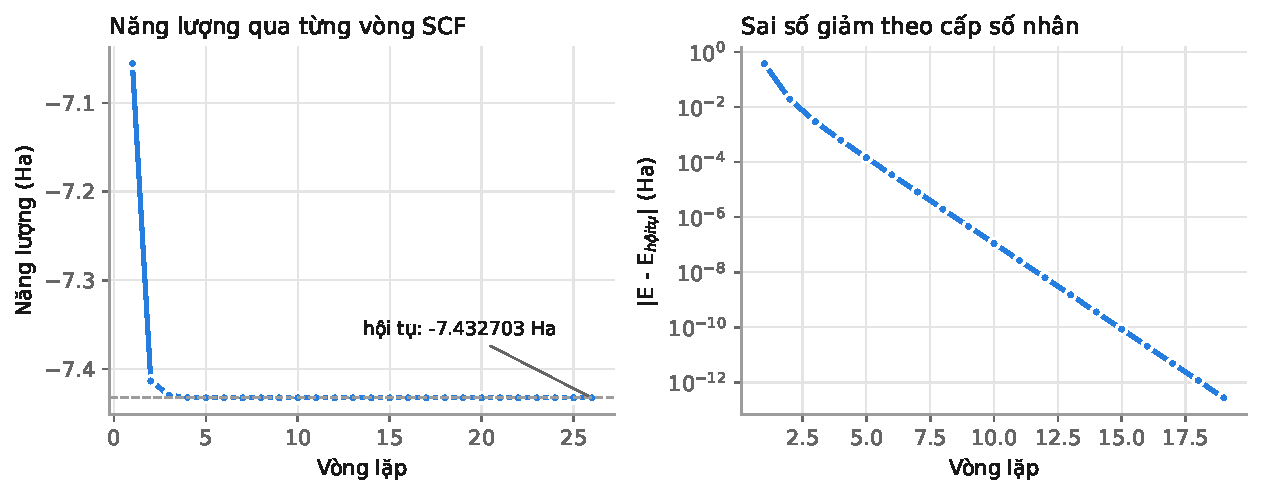
\includegraphics[width=\textwidth]{02_scf_hoi_tu.pdf}
\caption{Vòng lặp SCF tự viết cho Li (UHF/cc-pCVTZ). Trái: năng lượng giảm từ $-7.056\Ha$ (vòng 1) và ổn định gần như ngay lập tức. Phải: sai số so với giá trị hội tụ giảm theo cấp số nhân, mỗi vòng khoảng 3--4 lần, cho tới giới hạn làm tròn của máy tính. (Script \code{02\_hartree\_fock.py})}
\label{fig:scf}
\end{figure}

\begin{hieulam}[``tự hợp'' nghĩa là ``đúng'']
Tự hợp chỉ có nghĩa là lời giải tạo ra đúng cái trường mà nó đã giả định. Lời giải tự hợp của HF vẫn thiếu năng lượng tương quan. Ngoài ra vòng lặp có thể dao động hoặc rơi vào một nghiệm không phải thấp nhất. Các chương trình thực tế dùng kỹ thuật tăng tốc như DIIS \cite{Pulay1980} để hội tụ nhanh và ổn định hơn.
\end{hieulam}

\section{Tập cơ sở: xếp Lego để vẽ orbital}\label{sec:tapcoso}

\begin{eli5}[Lego]
Thay vì vẽ hình dạng orbital tự do (cần vô số điểm), ta ``xếp Lego'': orbital là tổng của một số khối có hình dạng cố định, nhân với các hệ số điều chỉnh được. Bộ khối đó gọi là \textbf{tập cơ sở} \en{basis set}. Càng nhiều khối và khối càng đa dạng, hình vẽ càng sát thật. Bài toán vi phân trở thành bài toán ma trận, loại bài toán máy tính giải rất giỏi.
\end{eli5}

\paragraph{Hàm Slater và hàm Gauss.}
Lựa chọn tự nhiên là \textbf{hàm kiểu Slater} (STO) $r^{n-1}e^{-\zeta r}Y_{lm}$, có đúng mũi nhọn ở hạt nhân và đuôi suy giảm như nghiệm thật. Nhưng tích phân bốn tâm của STO rất khó tính. Năm 1950, Boys đề xuất dùng \textbf{hàm kiểu Gauss} (GTO) $x^ay^bz^c\,e^{-\alpha r^2}$ \cite{Boys1950}. Hàm Gauss có hình dạng ``sai'' (đỉnh tròn thay vì nhọn, đuôi tắt quá nhanh), nhưng có một tính chất thần kỳ:
\[
e^{-\alpha|\vr-\mathbf A|^2}\,e^{-\beta|\vr-\mathbf B|^2}=e^{-\frac{\alpha\beta}{\alpha+\beta}|\mathbf A-\mathbf B|^2}\;e^{-(\alpha+\beta)|\vr-\mathbf P|^2},\quad \mathbf P=\frac{\alpha\mathbf A+\beta\mathbf B}{\alpha+\beta}.
\]
Tích của hai hàm Gauss đặt ở hai tâm là một hàm Gauss đặt ở tâm thứ ba. Nhờ vậy mọi tích phân đều tính được bằng công thức, rất nhanh. Dùng nhiều hàm Gauss vẫn rẻ hơn dùng ít hàm Slater. Gần như mọi chương trình hóa lượng tử hiện nay dùng hàm Gauss.

\paragraph{Các họ tập cơ sở.}
\begin{itemize}
\item \textbf{STO-3G} \cite{Hehre1969}: tập ``cực tiểu''. Mỗi orbital nguyên tử được xấp xỉ bằng 3 hàm Gauss. Li có 5 hàm (1s, 2s, 2p$_{x,y,z}$).
\item \textbf{6-31G}: lớp hóa trị được ``tách đôi'' để linh hoạt hơn. Li có 9 hàm.
\item \textbf{cc-pVXZ} (X = D, T, Q, 5 ứng với 2, 3, 4, 5) \cite{Dunning1989,Prascher2011}: họ ``tương quan nhất quán'' \en{correlation-consistent} của Dunning. Mỗi bậc X thêm một lớp hàm có mômen động lượng cao hơn. Li có 14, 30, 55, 91 hàm.
\item \textbf{cc-pCVXZ}: thêm các hàm ``chặt'' (tập trung gần hạt nhân) để mô tả tương quan của electron lõi. Li có 18, 43, 84 hàm. Chương~\ref{ch:sauhf} sẽ cho thấy với Li, loại này là \emph{bắt buộc}.
\end{itemize}

\begin{figure}[h]
\centering
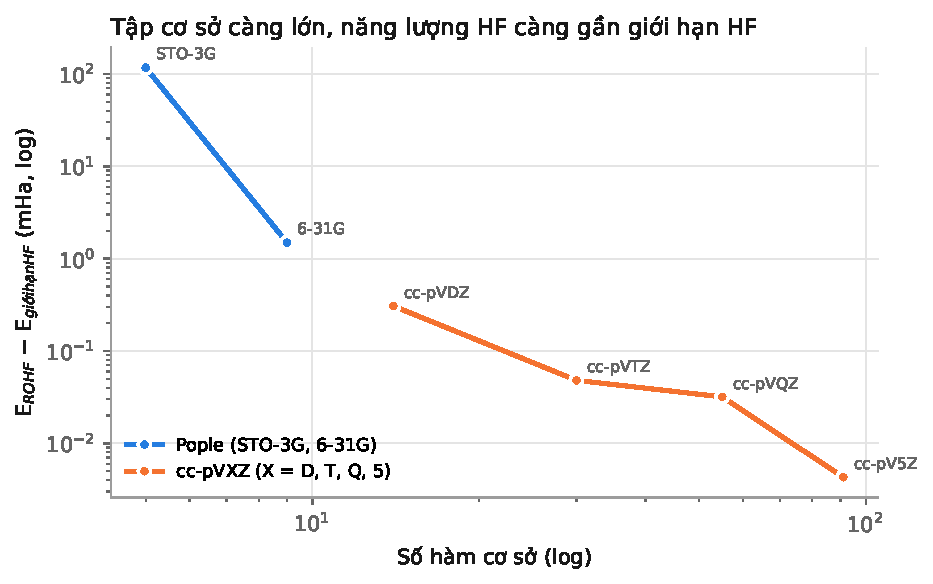
\includegraphics[width=0.82\textwidth]{02_hoi_tu_tap_co_so.pdf}
\caption{Năng lượng ROHF của Li hội tụ về giới hạn HF ($-7.432\,727\Ha$) khi tập cơ sở lớn dần. STO-3G sai $117\mHa$, cc-pV5Z chỉ còn sai $0.004\mHa$. (Script \code{02\_hartree\_fock.py})}
\label{fig:coso}
\end{figure}

\begin{table}[h]
\centering\small
\caption{Năng lượng ROHF của Li theo tập cơ sở (tính bằng code đi kèm). Các hàm lõi (cc-pCVXZ) hầu như không đổi năng lượng HF.}
\label{tab:hfcoso}
\begin{tabular}{@{}lrrr@{}}
\toprule
Tập cơ sở & Số hàm & $E_{\rm ROHF}$ (Ha) & Sai số so với giới hạn HF (mHa) \\
\midrule
STO-3G & 5 & $-7.315\,526$ & $117.20$ \\
6-31G & 9 & $-7.431\,235$ & $1.49$ \\
cc-pVDZ & 14 & $-7.432\,420$ & $0.307$ \\
cc-pVTZ & 30 & $-7.432\,679$ & $0.048$ \\
cc-pVQZ & 55 & $-7.432\,695$ & $0.032$ \\
cc-pV5Z & 91 & $-7.432\,723$ & $0.004$ \\
cc-pCVQZ & 84 & $-7.432\,695$ & $0.032$ \\
aug-cc-pCVQZ & 109 & $-7.432\,696$ & $0.031$ \\
\midrule
Giới hạn HF \cite{KogaThakkar1996} & $\infty$ & $-7.432\,727$ & 0 \\
\bottomrule
\end{tabular}
\end{table}

Năng lượng HF hội tụ rất nhanh theo tập cơ sở (gần như theo hàm mũ của X). Ta sẽ thấy ở chương sau rằng năng lượng tương quan hội tụ \emph{chậm hơn nhiều}, chỉ như $X^{-3}$, vì phải vẽ mũi nhọn electron--electron bằng các ``khối Lego'' tròn trịa.

\section{Vỏ mở: ROHF và UHF}

Li có một electron lẻ, nên có hai cách làm HF:
\begin{itemize}
\item \textbf{ROHF} \en{restricted open-shell}: hai electron 1s dùng \emph{chung} một orbital không gian. Hàm sóng có spin toàn phần đúng bằng $\tfrac12$.
\item \textbf{UHF} \en{unrestricted}: cho phép orbital của electron spin lên và spin xuống khác nhau. Năng lượng thấp hơn (vì linh hoạt hơn), nhưng hàm sóng không còn là trạng thái spin ``sạch''.
\end{itemize}

Trong UHF, electron 2s$\uparrow$ có tương tác trao đổi với 1s$\uparrow$ nhưng không với 1s$\downarrow$, nên hai orbital 1s tách nhau một chút. Năng lượng orbital tính được: $\varepsilon_{1s\uparrow}=-2.4867\Ha$ và $\varepsilon_{1s\downarrow}=-2.4687\Ha$. Hiện tượng này gọi là \textbf{phân cực spin lõi}. Nó có thật: nó làm mật độ spin tại hạt nhân khác 0 và ảnh hưởng tới phổ siêu tinh tế đo được của Li \cite{Sachs1960}.

\begin{congthuc}[nhiễm bẩn spin]
Với trạng thái doublet thuần, $\langle\hat S^2\rangle=S(S+1)=0.75$. Hàm UHF có thể lẫn một chút trạng thái quartet ($S=\tfrac32$), làm $\langle\hat S^2\rangle>0.75$. Với Li/aug-cc-pCVQZ, code cho:
\[
E_{\rm ROHF}=-7.432\,696\Ha,\quad E_{\rm UHF}=-7.432\,720\Ha,\quad \langle\hat S^2\rangle_{\rm UHF}=0.750\,016 .
\]
Nhiễm bẩn rất nhỏ, và UHF chỉ thấp hơn ROHF $0.024\mHa$. Với Li, chọn cách nào cũng được. Với các hệ khác (phân tử bị kéo giãn, gốc tự do) nhiễm bẩn spin có thể lớn và gây sai lệch nghiêm trọng.
\end{congthuc}

\section{Định lý Koopmans: năng lượng orbital có nghĩa gì?}

\begin{eli5}[chụp ảnh tập thể]
Bạn muốn ước tính ``giá'' của việc rút một người ra khỏi bức ảnh tập thể. Cách nhanh nhất: giả sử những người còn lại đứng yên không nhúc nhích. Đó là ý tưởng của định lý Koopmans. Ngoài đời, khi một người rời đi, những người còn lại sẽ xê dịch (gọi là \emph{hồi phục orbital}), và cách họ né nhau cũng thay đổi (tương quan).
\end{eli5}

\begin{congthuc}[định lý Koopmans]
Nếu các orbital còn lại ``đông cứng'' khi lấy electron khỏi orbital $a$, năng lượng ion hóa bằng trừ năng lượng orbital \cite{Koopmans1934}:
\[
\text{IE}_a\approx-\varepsilon_a .
\]
\end{congthuc}

\begin{table}[h]
\centering\small
\caption{Năng lượng ion hóa thứ nhất của Li (tính bằng code, tập cơ sở aug-cc-pCVQZ).}
\label{tab:koopmans}
\begin{tabular}{@{}lrr@{}}
\toprule
Cách tính & IE (eV) & Sai số (eV) \\
\midrule
Koopmans: $-\varepsilon_{2s}$ (UHF) & 5.343 & $-0.049$ \\
$\Delta$SCF: $E_{\rm HF}(\text{Li}^+)-E_{\rm HF}(\text{Li})$ & 5.343 & $-0.049$ \\
Từ năng lượng chính xác: $E(\text{Li}^+)-E(\text{Li})$ & 5.392 & $+0.000$ \\
Thực nghiệm \cite{NIST-ASD} & 5.392 & --- \\
\bottomrule
\end{tabular}
\end{table}

Bảng~\ref{tab:koopmans} kể một câu chuyện thú vị. Koopmans và $\Delta$SCF gần như trùng nhau, nghĩa là hiệu ứng hồi phục orbital rất nhỏ: rút electron 2s ở xa ra hầu như không làm lõi 1s$^2$ co lại. Cả hai đều thiếu đúng $0.050\eV$. Con số này chính là \emph{hiệu năng lượng tương quan} giữa Li và Li$^+$: $\Ecorr(\text{Li})-\Ecorr(\text{Li}^+)=-45.33-(-43.50)=-1.83\mHa=-0.050\eV$. Khi dùng năng lượng chính xác, sai số biến mất. Năm 1936, James và Coolidge đã nhận ra đúng sai số $0.05\eV$ này khi dùng hàm sóng không tính tới chuyển động tương đối giữa electron lớp K và lớp L \cite{JamesCoolidge1936}.

\section{Hartree--Fock bỏ sót gì?}
HF cho Li năng lượng $-7.432\,727\Ha$, đúng 99.4\% năng lượng toàn phần. Nhưng như đã nói ở chương~\ref{ch:hatdongnhat}, phần 0.6\% còn thiếu ($45.3\mHa$) gấp 28 lần độ chính xác hóa học. Phần thiếu đến từ việc các electron \emph{khác spin} chuyển động hoàn toàn độc lập trong HF: hai electron 1s có thể ``đứng'' cùng một chỗ với xác suất bằng tích xác suất riêng lẻ, trong khi thực tế chúng né nhau. Chương tiếp theo trình bày các cách sửa lỗi này một cách có hệ thống.

\begin{ghinho}
\begin{itemize}
\item HF tìm định thức Slater tốt nhất. Mỗi electron chuyển động trong trường trung bình của hạt nhân và các electron khác. Phương trình phi tuyến nên phải lặp tới tự hợp (SCF).
\item Năng lượng gồm phần Coulomb $J$ (cổ điển) và phần trao đổi $-K$ (chỉ giữa electron cùng spin, thuần lượng tử). HF không có lỗi tự tương tác.
\item Orbital được biểu diễn bằng tập cơ sở Gauss; phương trình thành bài toán ma trận $\mathbf{FC}=\mathbf{SC}\boldsymbol\varepsilon$. HF hội tụ nhanh theo tập cơ sở.
\item Với Li: $\EHF=-7.432\,727\Ha$; Koopmans cho IE $=5.34\eV$ (thực nghiệm 5.39). Phần thiếu là tương quan, chủ yếu giữa hai electron 1s khác spin.
\end{itemize}
\end{ghinho}
